\documentclass[12pt,letterpaper]{exam}
\usepackage[lmargin=1in,rmargin=1in,tmargin=1in,bmargin=1in]{geometry}
\usepackage{../style/exams}

% -------------------
% Course & Exam Information
% -------------------
\newcommand{\course}{MAT 108: Exam 2}
\renewcommand{\term}{Spring -- 2023}
\newcommand{\examdate}{04/03/2023}
\newcommand{\timelimit}{85 Minutes}

\setbool{hideans}{true} % Student: True; Instructor: False

% -------------------
% Content
% -------------------
\begin{document}

\examtitle
\instructions{Write your name on the appropriate line on the exam cover sheet. This exam contains \numpages\ pages (including this cover page) and \numquestions\ questions. Check that you have every page of the exam. Answer the questions in the spaces provided on the question sheets. Be sure to answer every part of each question and show all your work. If you run out of room for an answer, continue on the back of the page --- being sure to indicate the problem number.} 
\scores
\bottomline
\newpage

% ---------
% Questions
% ---------
\begin{questions}

% Question 1
\newpage
\question[15] A sports analyst is testing the claim whether taller basketball players are inherently better than shorter players. The analyst creates a linear regression to predict the number of baskets scored in 60~seconds by players between 75~in and 86~in. The model is found to be $\widehat{y}= 1.2x - 69.7$ with $r= 0.8691$. 
	\begin{enumerate}[(a)]
	\item Predict the number of shots made in the given time by a player with a height of 78~in. \pvspace{2cm}
	
	\item Which of the following scatterplots is the most likely to represent the data and the model? \par
		\begin{figure}[!ht]
		\centering
		\hfill
		\begin{subfigure}[b]{0.3\textwidth}
		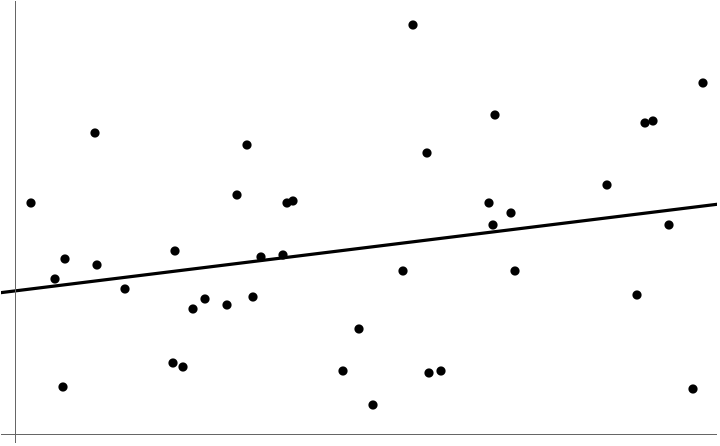
\includegraphics[width=\textwidth]{plot1.png}
		\caption{}
		\end{subfigure}
		\hfill
		\begin{subfigure}[b]{0.3\textwidth}
		\includegraphics[width=\textwidth]{{plot2.png}}
		\caption{}
		\end{subfigure} \par
		\hfill
		\begin{subfigure}[b]{0.3\textwidth}
		\includegraphics[width=\textwidth]{{plot3.png}}
		\caption{}
		\end{subfigure}
		\hfill
		\begin{subfigure}[b]{0.3\textwidth}
		\includegraphics[width=\textwidth]{{plot4.png}}
		\caption{}
		\end{subfigure}
		\end{figure} \pvspace{1.3cm}
	
	\item Find the value of the coefficient of determination. \pvspace{3cm}
	
	\item Should one use this model to predict the shots made by someone with a height of 65~in?	
	\end{enumerate}



% Question 2
\newpage
\question[10] An administrator is trying to determine if there is any correlation between student success and a new support program offered by the college. They gather the following data:
	\begin{table}[!ht]
	\centering
	\begin{tabular}{|l||c|c|c|} \hline
	& Program Participant & Non-Participant & Total \\ \hline \hline
	Graduated & 87 & 453 & 540 \\ \hline
	Not Graduated & 13 & 187 & 200 \\ \hline \hline
	Total & 100 & 640 & 740 \\ \hline
	\end{tabular}
	\end{table}

\begin{enumerate}[(a)]
\item Find the probability that a randomly selected student was a program participant and graduated.
\item Find the probability that a randomly selected student participated in the program or graduated. 
\item Find the probability that a randomly selected program participant graduated. 
\end{enumerate}



% Question 3
\newpage
\question[10] The English Department at a small college offers two non-standard degrees: playwriting and copy editing. There are 63~students in the English Department. There are 8~playwriting majors, 6 copy editing majors, including 2 double majors in playwriting and copy editing. 
	\begin{enumerate}[(a)]
	\item What is the probability that a randomly selected student in this department does not major in playwriting or copy editing?
	\item What is the probability that a randomly selected student in this department majors in playwriting but not copy editing. 
	\item If a student majors in copy editing, what is the probability they also major playwriting?
	\end{enumerate}



% Question 4
\newpage
\question[10] Not all people that work in the public sector have a college degree. Approximately 42\% of students go to college. Of those people that go to college, approximately 14\% work in the public sector while 22\% of non-college educated people work in the public sector. 
	\begin{enumerate}[(a)]
	\item What percent of people work in the public sector?
	\item What percent of people work in the public sector or go to college?
	\item If a person works in the public sector, what is the probability they hold a college degree?
	\end{enumerate}



% Question 5
\newpage
\question[10] A local casino sells a special `in-house' scratch ticket for \$1 that primarily offers discounts for various offerings around the hotel. However, there is a 1 in 500,000 chance to win \$100,000 and a 1 in 1,000 chance to win \$100. Find the expected net payout buying these scratch tickets. Is the sale of tickets for the casino a `wise' financial decision? 



% Question 6
\newpage
\question[15] Data Science is one of the `hottest' fields of the last 15~years. The average salary for a data scientist is \$137,000. Suppose that these salaries are normally distributed with standard deviation \$39,000. 
	\begin{enumerate}[(a)]
	\item Find the percentage of data scientists that make less than \$100,000 per year.
	\item Find the percentage of data scientists that make more than \$100,000 per year.
	\item Find the probability that if you take a random sample of 5~data scientists that their average salary is less than \$100,000.  
	\end{enumerate}



% Question 7
\newpage
\question[10] A dual liberal arts college and conservatory accepts approximately 4,000 students each year. Of these students, approximately 15\% of these accepted students are admitted into the conservatory. You take a simple random sample of 13~students.
	\begin{enumerate}[(a)]
	\item Find the probability that at most 4 of these students were admitted to the conservatory. 
	\item Find the probability that more than 5 of these students were admitted to the conservatory. 
	\item Find the probability that at least one of these students was admitted to the conservatory. 
	\end{enumerate}



% Question 8
\newpage
\question[10] A medical researcher is examining the relation between vitamin levels in blood and cancer risks. Based on a sample of 200~cancer-free individuals, an average of 11.7~mg/L of a particular vitamin were found in patients blood. Assuming a standard deviation of $\sigma= 3.65 \text{ mg/L}$, find a 92\% confidence interval for the level of vitamin found in cancer-free blood.  



% Question 9
\newpage
\question[10] An architect is working on plans for an academic building. For a large lecture hall, the architect is trying to determine how many left handed sets should be placed in the room. The lecture hall will have 250~seats. Research suggests that approximately 11\% of individuals are left-handed. The architect decides to place 35 left handed seats in the room. Use the normal approximation to find the probability that if the lecture hall is full that there will be at most 35 left handed students in the room. 


\end{questions}
\end{document}